
\question(20分)已知控制系统结构图如下所示,求 $C(s),\hat{C}(s)$

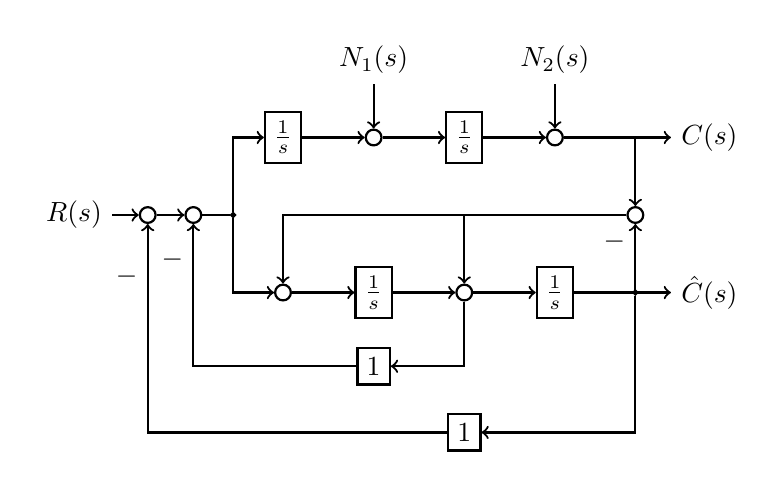
\begin{tikzpicture}[scale=1, thick] 
\tikzstyle{block} = [draw,rectangle,thick,minimum height=1em,minimum width=1em]
\tikzstyle{sum} = [draw,circle,inner sep=0mm,minimum size=2mm]
\tikzstyle{branch} = [draw,fill,circle,inner sep=0pt,minimum size=0.5mm]
\tikzstyle{connector} = [->,thick]
\matrix[ampersand replacement=\&, row sep=1em, column sep=1em]{
	\&\&\&\&\& \node(n1){$N_1(s)$};\&\&\node(n2){$N_2(s)$}; \\
	
	\&\&\&\& \node[block](g1){$\frac{1}{s}$}; \& \node[sum](pn1) {}; \& \node[block] (g2){$\frac{1}{s}$}; \& \node[sum](pn2) {};  \&
	\& \node[] (c){$C(s)$};\\
	
	\node[] (r) {$R(s)$}; \& 
	\node[sum](pe1) {};\&
	\node[sum](pe2) {};\&
	\node[branch] (b1) {} ; \&\&\&\&\&
	\node[sum](pe3) {};\\
	
	\&\&\&\& \node[sum](ps1) {}; \& 
	\node[block](g3){$\frac{1}{s}$}; \& 
	\node[sum](ps2) {}; \& \node[block](g4){$\frac{1}{s}$};\&
	\node[branch] (b2) {} ;  \& \node[] (hatc){$\hat{C}(s)$}; \\
	
	\&\&\&\&\& \node[block](h1) {$1$}; \\
	\&\&\&\&\&\& \node[block](h2){$1$}; \\
};
\draw [connector] (n1) -- (pn1);
\draw [connector] (n2) -- (pn2);
\draw [connector] (r) -- (pe1);
\draw [connector] (pe1) -- (pe2);
\draw [thick] (pe2) -- (b1);
\draw [connector] (b1) |- (g1);
\draw [connector] (b1) |- (ps1);
\draw [connector] (ps1) -- (g3);
\draw [connector] (g1) -- (pn1);
\draw [connector] (pn1) -- (g2);
\draw [connector] (g3) -- (ps2);
\draw [connector] (ps2) -- (g4);
\draw [connector] (g2) -- (pn2);
\draw [connector] (pn2) -| (pe3);
\draw [connector] (pn2) -- (c);
\draw [connector] (g4) -|   node[very near end,left] {$-$} (pe3);
\draw [connector] (g4) -- (hatc);
\draw [connector] (pe3) -| (ps1);
\draw [connector] (pe3) -| (ps2);
\draw [connector] (ps2) |- (h1);
\draw [connector] (b2) |- (h2);
\draw [connector] (h1) -|  node[very near end,left] {$-$} (pe2);
\draw [connector] (h2) -|  node[very near end,left] {$-$} (pe1);
\end{tikzpicture} 

\onlyanswer
{
答:设 $E(s)=C(s)-\hat{C}(s)$,得:
\begin{align*}
s\hat{C}(s) &= \frac{R(S)-\hat{C}(s)-s\hat{C}(s)+E(s)}{s}+E(s) \\
s\hat{C}(s)+\hat{C}(s)+\frac{\hat{C}(s)}{s}&= \frac{R(s)+sE(s)+E(s)}{s}\\
(s^2+s+1)\hat{C}(s) &=R(s)+(s+1)E(s)\\
\hat{C}(s) &=\frac{R(s)+(s+1)E(s)}{s^2+s+1}
\end{align*}
及:
\begin{align*}
C(s) &= \frac{R(S)-\hat{C}(s)-s\hat{C}(s)}{s^2}+\frac{N_1(s)}{s}+N_2(s)\\
s^2 C(s) &= R(s)-(s+1)\hat{C}(s)+sN_1(s)+s^2 N_2(s)\\
s^2 C(s) &= R(s)-(s+1)(C(s)-E(s))+sN_1(s)+s^2 N_2(s)\\
(s^2+s+1) C(s) &= R(s)+(s+1)E(s)+sN_1(s)+s^2 N_2(s)\\
 C(s) &= \frac{R(s)+(s+1)E(s)+sN_1(s)+s^2 N_2(s)}{s^2+s+1}
\end{align*}

得:
\begin{align*}
\hat{C}(s) &=\frac{R(s)+(s+1)E(s)}{s^2+s+1}\\
 C(s) &= \frac{R(s)+(s+1)E(s)+sN_1(s)+s^2 N_2(s)}{s^2+s+1}\\
E(s) &=\frac{sN_1(s)+s^2 N_2(s)}{s^2+s+1}\\
\hat{C}(s) &=\frac{R(s)}{s^2+s+1}+\frac{(s+1)(sN_1(s)+s^2 N_2(s))}{(s^2+s+1)^2}\\
C(s) &= \frac{R(s)+sN_1(s)+s^2 N_2(s)}{s^2+s+1}+\frac{(s+1)(sN_1(s)+s^2 N_2(s))}{(s^2+s+1)^2}
\end{align*}

另一种方法:
\begin{align*}
(s^2+s+1)\hat{C}(s) &=R(s)+(s+1)(C(s)-\hat{C}(s))\\
(s^2+2s+2)\hat{C}(s) &=R(s)+(s+1)C(s)
\end{align*}
及:
\begin{align*}
C(s) &= \frac{R(S)-\hat{C}(s)-s\hat{C}(s)}{s^2}+\frac{N_1(s)}{s}+N_2(s)\\
s^2 C(s) &= R(s)-(s+1)\hat{C}(s)+sN_1(s)+s^2 N_2(s)
\end{align*}
求解:
\begin{align*}
s^2(s^2+2s+2)\hat{C}(s) &=s^2R(s)+s^2(s+1)C(s)\\
(s+1)s^2 C(s) &= (s+1)R(s)-(s+1)^2\hat{C}(s)+(s+1)sN_1(s)+(s+1)s^2 N_2(s)\\
s^2(s^2+2s+2)\hat{C}(s) &=(s^2+s+1)R(s)-(s+1)^2\hat{C}(s)+(s+1)sN_1(s)+(s+1)s^2 N_2(s)\\
(s^4+2s^3+2s^2+(s+1)^2)\hat{C}(s)  &=(s^2+s+1)R(s)+(s+1)sN_1(s)+(s+1)s^2 N_2(s) \\
\hat{C}(s)  &=\frac{(s^2+s+1)R(s)+(s+1)sN_1(s)+(s+1)s^2 N_2(s)}{s^4+2s^3+3s^2+2s+1}
\end{align*}
}

\question(20分)已知系统结构图如下:

\begin{tikzpicture}[scale=1, thick] 

\tikzstyle{block} = [draw,rectangle,thick,minimum height=1em,minimum width=1em]
\tikzstyle{sum} = [draw,circle,inner sep=0mm,minimum size=2mm]
\tikzstyle{branch} = [draw,circle,fill,inner sep=0pt,minimum size=0.5pt]
\tikzstyle{connector} = [->,thick]

\def\p(#1){\node[sum](p#1){};}
\def\b(#1){\node[branch](b#1){};}
\def\gr{\node[block](gr){ $k_2 s$ };}
\def\gk{\node[block](gk){ $k_1$ };}
\def\gh{\node[block](gh){$1$};}
\def\guv{\node[block](guv){$\dfrac{1}{ s}$};}
\def\gvy{\node[block](gvy){$\dfrac{1}{ s}$};}
\def\c{\node(c){$Y(s)$}; }
\def\r{\node(r){$R(s)$};}
\matrix[ampersand replacement=\&, row sep=1em, column sep=2em]{
	\&        \&   \gr    \\
	\r   \& \b(r) \&   \p(e)  \& \p(u)   \&\guv  \& \b(v)  \& \gvy    \& \b(y)  \&  \c\\
	\&         \&            \&          \& \gk\\
	\&         \&            \&           \& \gh\\
};

\draw [connector] (r) -- (pe);
\draw [connector] (br) |-(gr);
\draw [connector] (pe) -- node[midway,above] {$E(s)$}(pu);
\draw [connector] (gr) -|(pu);
\draw [connector] (pu) -- node[midway,above] {$U(s)$}(guv);
\draw [connector] (guv) -- node[midway,above] {$V(s)$}(gvy);
\draw [connector] (gvy) --(c);
\draw [connector]( bv) |-(gk);
\draw [connector] (gk) -| node[near end,left] {$-$} (pu);
\draw [connector] (by) |-(gh);
\draw [connector] (gh) -| node[very near end,left] {$-$} (pe);

\let\b\undefined
\let\p\donothing
\end{tikzpicture} 

写出微分方程组;求解当 $v(0)=1,y(0)=1,r(t)=t$ 时的稳态误差;分析当$k_1$取何值时系统为临界阻尼系统。

\onlyanswer
{
答:系统微分方程组:
\begin{align*}
\dot{y}(t) &=v(t) \\
\dot{v}(t) &=k_2\dot{r}(t)+r(t)-y(t)+k_1 v(t)
\end{align*}
考虑到初始条件,进行Laplace变换,得:
\begin{align*}
sY(s)-y(0) &=V(s) \\
sY(s)-1 &=V(s) \\
sV(s)-v(0) &=k_2 sR(s)+R(s)-Y(s)-k_1 V(s)\\
(s+k_1)V(s)-1 &=k_2 sR(s)+R(s)-Y(s)\\
s(s+k_1) Y(s)-(s+k_1)-1 &= k_2 sR(s)+R(s)-Y(s)\\
Y(s) &=\frac{k_2 sR(s)+R(s)+s+k_1+1}{s(s+k_1)+1}\\
E(s) &=R(s)-Y(s) \\
&=\frac{s(s+k_1)R(s)-k_2 sR(s)-s-k_1-1}{s(s+k_1)+1}
\end{align*}
当$k_1>0$时,系统稳定。当$k_1=2$时为临界阻尼系统。
$r(t)=t$时:
\begin{align*}
\lim_{s\to 0}sE(s) &=\frac{(s+k_1)-k_2 -s^2-k_1s-s}{s(s+k_1)+1}\\
&=k_1-k_2
\end{align*}
}

\question(20分)已知单位负反馈系统开环传递函数:
$$G(s)=\frac{1}{s^3+3s^2+s+1}$$
分析闭环系统稳定性与稳定裕度。


\onlyanswer
{
	答:
	系统闭环传递函数为:
	$$\Phi(s)=\frac{1}{s^3+3s^2+s+2}$$
	Routh表:
$$
\begin{matrix}
 s^3  & 1 & 1 \\
 s^2  & 3 & 2 \\
 s^1  & \frac{1}{3}  & 0 \\
 s^0  & 2
\end{matrix}
$$
可知闭环系统稳定。

计算相角裕度:
\begin{align*}
|G(j\omega_c)|&=1\\
\omega_c &=0\\
\gamma &=180^\circ
\end{align*}

原系统穿越频率$\omega_x$与开环传递函数为
$$G'(s)=\frac{k}{s^3+3s^2+s+1}$$
的系统相同。当选取合适的$k$使Nyquist曲线穿过(-1+0j)时,此时闭环系统
	$$\Phi'(s)=\frac{1}{s^3+3s^2+s+1+k}$$
存在纯虚根,可通过Routh判据计算出此时的$\omega_x$。
	Routh表:
	$$
	\begin{matrix}
	s^3  & 1 & 1 \\
	s^2  & 3 & 1+k \\
	s^1  & 1-\frac{1+k}{3} & 0 
	\end{matrix}
	$$
令$k=2$,则出现全零行,构建辅助方程$3s^2+3=0$,得:
\begin{align*}
\lambda &=\pm 1j \\
\omega_x &=1 \\
|G(j\omega_x )| &=\frac{1}{|-1j-3+1j+1|} \\
 &=\frac{1}{2} \\
h &= 2
\end{align*}


}

\question(20分)单位负反馈系统开环传递函数:
$$G(s)=\frac{k(s^2+a)}{(s+b)^2}$$
$a,b$均为实数且$b\neq 0$。绘制$k\in (-\infty,0)\cup (0,+\infty)$时系统的根轨迹并分析其形状。

\onlyanswer
{
	答:
	若$s$闭环系统极点,则有$1+G(s)=0$,可知$G(s)$的虚部为零。
	\begin{align*}
	0 &=\Im[ G(s)] \\
	&= \Im\left[\frac{k((x+i y)^2+a)}{((x+i y)+b)^2}\right]\\
	&=\frac{k(2xy((x+b)^2-y^2)-2(x+b)y(-y^2+x^2+a))}{(y^2+(x+b)^2)^2}\\
	0&=(2xy((x+b)^2-y^2)-2(x+b)y(-y^2+x^2+a))\\
	&=y(by^2+bx^2+b^2x-ax-ab)\\
	&=y\left(y^2+(x+\frac{b^2-a}{2b})^2-\frac{(b^2-a)^2}{4b^2}-a\right)\\
	&=y\left(y^2+(x+\frac{b^2-a}{2b})^2-\frac{(b^2+a)^2}{4b^2}\right)
	\end{align*}
	因此,根轨迹在实轴上或者在圆心:$(-\frac{b^2-a}{2b}+0i)$、半径:$|\frac{b^2+a}{2b}|$的圆上。
	
	$a>0,b>0$时,根轨迹如下:
	
	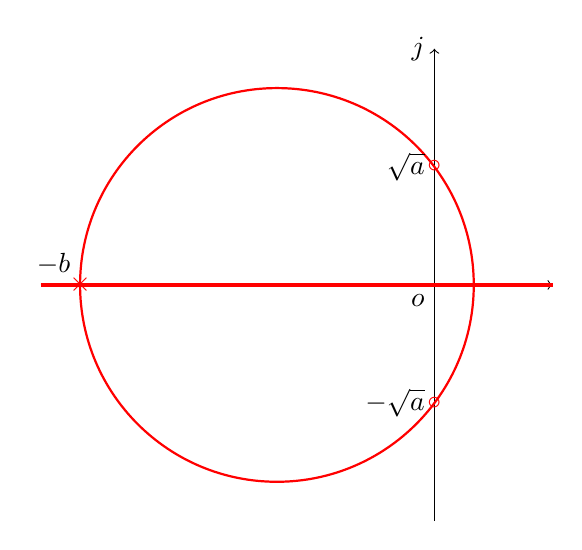
\begin{tikzpicture}
	\coordinate (o) at (0,0);
	\coordinate (ox) at (1.5,0);
	\draw[->] (-5,0) -- (ox);
	\draw[->] (0,-3) -- (0,3);
	\draw (o) node[below left] {$o$};
	\draw[thick,red] (-4.5,0) node {$\times$};
	\draw[thick,red] (0,1.5) node {$\circ$};
	\draw[thick,red] (0,-1.5) node {$\circ$};
	\draw [red,thick] (0.5,0) arc (0:360:2.5);
	\draw [red,very thick] (-5,0)--(1.5,0);
	\draw (0,3) node[left] {$j$};
	\draw (-4.5,0) node[above left] {$-b$};
	\draw (0,1.5) node[left ] {$\sqrt{a}$};
	\draw (0,-1.5) node[left ] {$-\sqrt{a}$};
	\end{tikzpicture}
	
	$-b^2<a<0,b>0$时,根轨迹如下:
	
	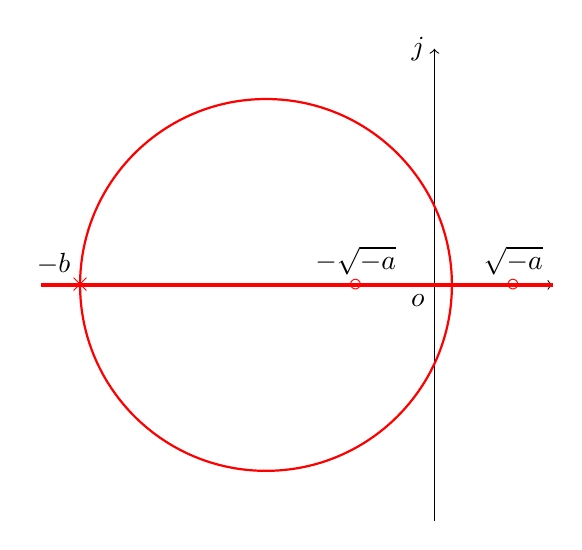
\begin{tikzpicture}
	\coordinate (o) at (0,0);
	\coordinate (ox) at (1.5,0);
	\draw[->] (-5,0) -- (ox);
	\draw[->] (0,-3) -- (0,3);
	\draw (o) node[below left] {$o$};
	\draw[thick,red] (-4.5,0) node {$\times$};
	\draw[thick,red] (1,0) node {$\circ$};
	\draw[thick,red] (-1,0) node {$\circ$};
	\draw [red,thick] (-4.5,0) arc (-180:180:85/36);
	\draw [red,very thick] (-5,0)--(1.5,0);
	\draw (0,3) node[left] {$j$};
	\draw (-4.5,0) node[above left] {$-b$};
	\draw (1,0) node[above ] {$\sqrt{-a}$};
	\draw (-1,0) node[above] {$-\sqrt{-a}$};
	\end{tikzpicture}
	
	$a<-b^2,b>0$时,根轨迹如下:
	
	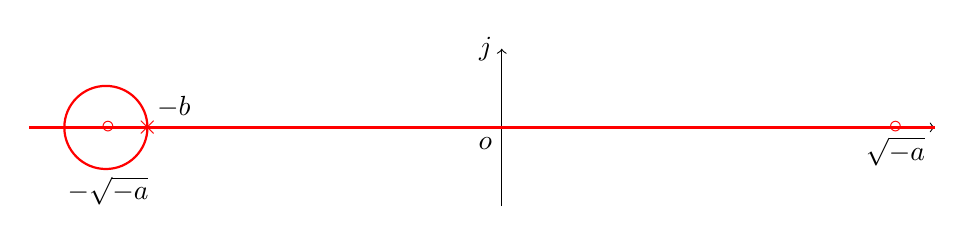
\begin{tikzpicture}
	\coordinate (o) at (0,0);
	\coordinate (ox) at (5.5,0);
	\draw[->] (-6,0) -- (ox);
	\draw[->] (0,-1) -- (0,1);
	\draw (o) node[below left] {$o$};
	\draw[thick,red] (-4.5,0) node {$\times$};
	\draw[thick,red] (5,0) node {$\circ$};
	\draw[thick,red] (-5,0) node {$\circ$};
	\draw [red,thick] (-4.5,0) arc (0:360:19/36);
	\draw [red,very thick] (-6,0)--(5.5,0);
	\draw (0,1) node[left] {$j$};
	\draw (-4.5,0) node[above right] {$-b$};
	\draw (5,0) node[below ] {$\sqrt{-a}$};
	\draw (-5,-0.5) node[below ] {$-\sqrt{-a}$};
	\end{tikzpicture}
	
	$a=-b^2,b>0$时,根轨迹如下:
	
	\begin{tikzpicture}
	\coordinate (o) at (0,0);
	\coordinate (ox) at (5.5,0);
	\draw[->] (-6,0) -- (ox);
	\draw[->] (0,-1) -- (0,1);
	\draw (o) node[below left] {$o$};
	\draw[thick,red] (-4.5,0) node {$\times$};
	\draw[thick,red] (-4.5,0) node {$\circ$};
	\draw[thick,red] (4.5,0) node {$\circ$};
	\draw [red,very thick] (-6,0)--(5.5,0);
	\draw (0,1) node[left] {$j$};
	\draw (-4.5,0) node[above] {$-b$};
	\draw (4.5,0) node[below ] {$\sqrt{-a}$};
	\draw (-4.5,0) node[below ] {$-\sqrt{-a}$};
	\end{tikzpicture}
	
	同理可得$b<0$时的根轨迹。
}


\question(20分)已知单位负反馈系统开环传递函数:
$$G(s)=\frac{k}{s}\cdot e^{-s}$$
求解使系统稳定的 $k$ 取值范围 (已知$k>0$)。

\onlyanswer
{
答:
\begin{align*}
G(j\omega)&=\frac{k}{j\omega}\cdot e^{j\omega}\\
\omega_c &= k \\
\omega_x &= \frac{\pi}{2}\\
\gamma  &=\frac{\pi}{2}-k
\end{align*}
因此,$k<\frac{\pi}{2}$时,系统稳定。
}